\documentclass[11pt,a4paper]{article}
% Packages
\usepackage{amsfonts}
\usepackage{amsmath}
\usepackage{amssymb}
\usepackage[hidelinks]{hyperref}
\usepackage{cleveref}
\usepackage{graphicx}
\usepackage[round]{natbib}
\usepackage{float,soul}
\usepackage{tikz}
\usepackage{caption}
\usepackage{tabularx}
\usepackage{xr}  % external document -- for supplements

\captionsetup[figure]{labelfont=bf,font=footnotesize}
\captionsetup[table]{labelfont=bf,font=footnotesize}

% Figure placement
\makeatletter
\def\fps@figure{tb}
\makeatother

% Newcommands
\DeclareMathSymbol{\shortminus}{\mathbin}{AMSa}{"39}  % useful for suffixes
\newcommand{\Ex}{\mathbb{E}}
\newcommand{\Var}{\mathrm{Var}}
\newcommand{\HW}{\mathrm{HW}}
\newcommand{\Bin}{\text{Binomial}}
\newcommand{\Uniform}{\text{Uniform}}
%\newcommand{\Normal}{\text{Normal}}
\newcommand{\Normal}{\mathcal{N}}
\newcommand{\Beta}{\text{Beta}}
\newcommand{\Exp}{\text{Exponential}}
\newcommand{\Gam}{\text{Gamma}}
\newcommand{\Bfun}{\mathrm{B}}
\newcommand{\eps}{\epsilon}
\newcommand{\logit}{\mathop{\mathrm{logit}}}
\newcommand{\Vx}{\mathcal{V}}



\usepackage{geometry}
\usepackage{authblk}
\externaldocument[m-]{paper}
\renewcommand{\thefigure}{S\arabic{figure}}
\renewcommand{\thesection}{S\arabic{section}}
\renewcommand{\thealgorithm}{S\arabic{algorithm}}

\begin{document}
\title{Supplement: Autopolyploid establishment through polygenic adaptation}
\author{Arthur Zwaenepoel}
\date{\vspace{-5ex}}
\maketitle
\tableofcontents
\clearpage

\section{Supplementary Figures}

\begin{figure}[H]
\centering
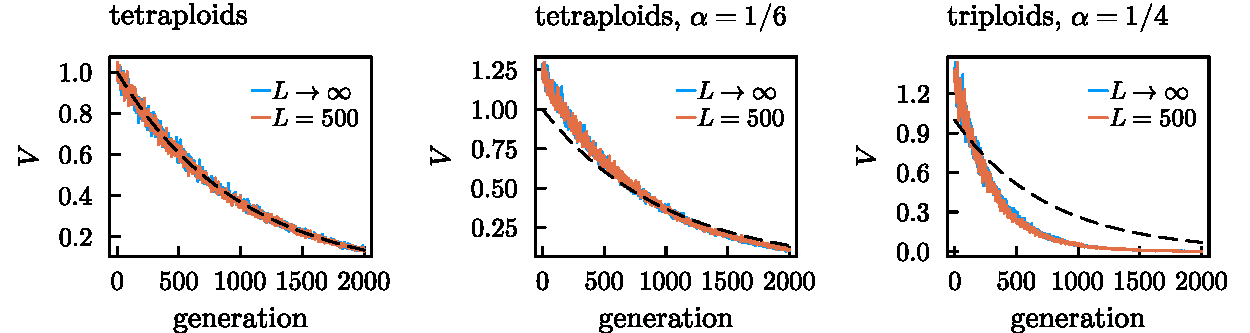
\includegraphics[width=\textwidth]{/home/arthur_z/dev/InfGenetics/doc/img/finsvsinf-polyploids-validation.pdf}
\caption{
Validation of the autotetraploid and triploid infinitesimal model by a
comparison against the discrete locus model with $L=500$ additive loci, showing
the average phenotypic variance in each generation averaged over 10 replicate
simulations for both models.
We assume the initial phenotypic variance to be one for all simulations, and
all replicates are initialized randomly in accordance with this initial
phenotypic variance.
Allelic effects for the discrete locus model are sampled from a Gaussian with
mean $0$ and variance $1/2L$.
\label{fig:fininf}}
\end{figure}

\begin{figure}[H]
\centering
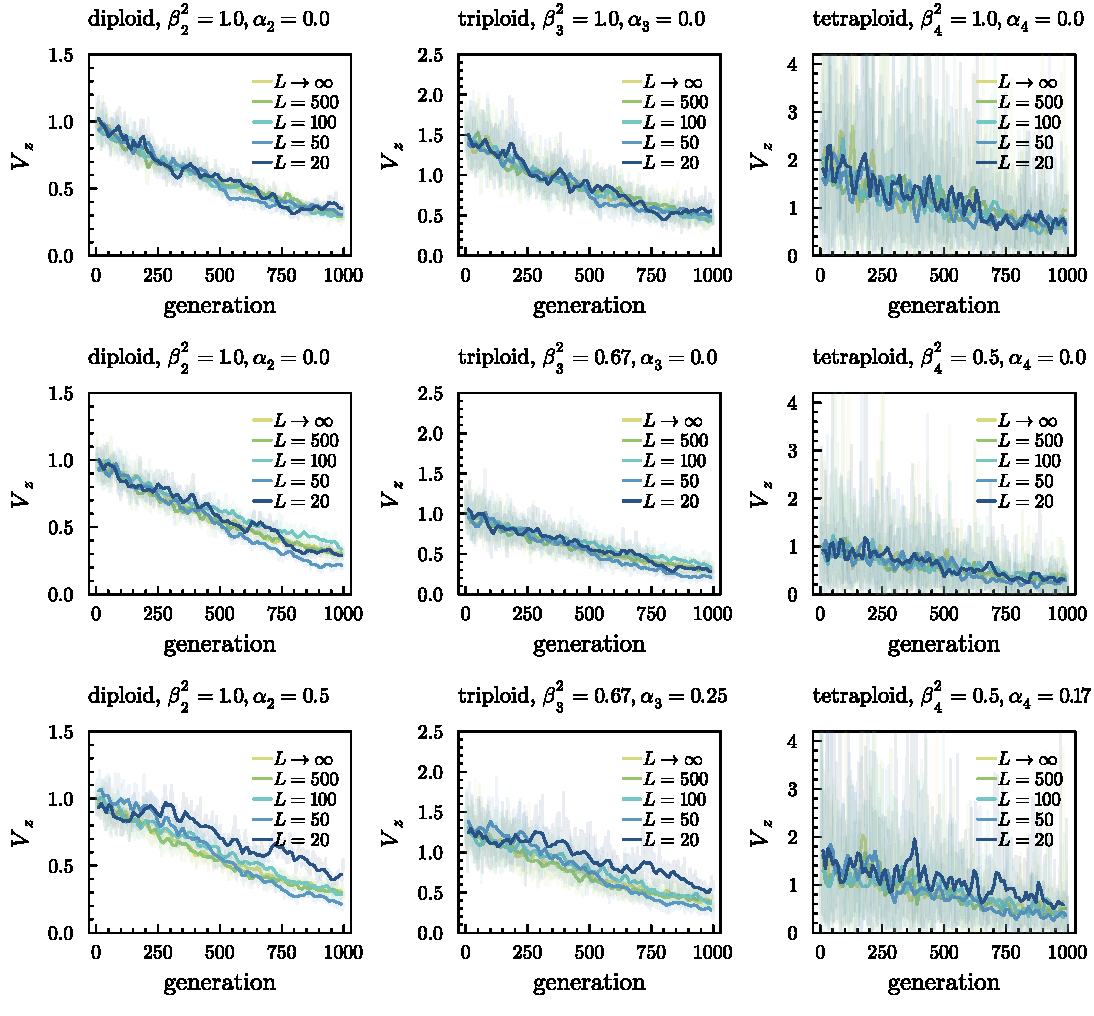
\includegraphics[width=\textwidth]{/home/arthur_z/vimwiki/build/img/2023-10-23/mixedploidy-Vz.pdf}
\caption{Comparison of the mixed-ploidy infinitesimal model with the
\(L\)-locus model, for \(L=500,100,50\) and \(20\). The decline in the
genetic variance \(V_z\) within each cytotype due to drift is shown. The
transparent lines show the complete simulation, whereas the solid line
shows the same data but smoothed in overlapping windows of 20
generations. We assume \(N=500, u=v=0.08\) and no selection. In the top
row where \(\beta_k^2=1, \alpha_k=0\), the equilibrium variance in the
absence of inbreeding in triploids is 2/3 that of diploids, and in
tetraploids it is twice that in diploids. In the middle row,
\(\beta_3^2=2/3\) and \(\beta_4^2=1/2\), so that the equilibrium
variance in the absence of inbreeding is equal across cytotypes. In the
bottom row, \(\alpha_2= \alpha_3 =1/2\) and \(\alpha_4=1/6\), causing an
immediate increase in the genetic variance in higher cytotypes, but also
accelerated inbreeding. \label{fig:vz}}
\end{figure}

\begin{figure}[H]
\centering
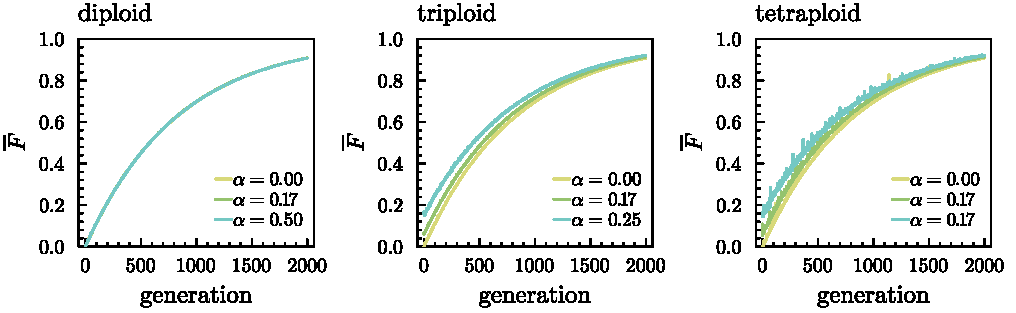
\includegraphics[width=\linewidth]{/home/arthur_z/vimwiki/build/img/2023-10-23/mixedploidy-F.pdf}
\caption{Average inbreeding coefficient \(\bar{F}\) in each cytotype in
a mixed-ploidy population for different values of \(\alpha\) (we assume
\(\alpha_k=\alpha\), where \(\alpha_k\) is the probability that a
diploid gamete produced by a \(k\)-ploid cytotype contains two copies of
the same parental gene at a random locus). We assume \(N=500, u=v=0.08\)
and no selection.}\label{fig:f1}
\end{figure}

\clearpage

\section{Supplementary Information}

\subsection{Deterministic mixed-ploidy model \label{sec:det}}

Let $g_k$ be the frequency of $k$-ploid gametes in the gamete pool, and let us
consider only haploid and diploid gametes, so that $g_2 = 1-g_1$.
Diploids produce unreduced gametes with probability $u$ and reduced ones with
probability $1-u$, triploids produce haploid and triploid gametes both with
probability $v$, and tetraploids produce reduced diploid gametes with
probability $(1-u)$ (we assume they produce, just like diploids, a proportion
$u$ of unreduced gametes, but these are assumed not to lead to viable offspring
and are ignored).
We get after one generation of random mating
  $$g_1' = \frac{(1-u)g_1^2 + 2vg_1g_2}{g_1^2 + 4vg_1g_2 + (1-u)g_2^2}.$$
We see that $g_1=0$ is always an equilibrium (no haploid gametes, tetraploids
take over).
Two more fixed points are obtained at
  \begin{equation}
  \tilde{g_1}, \tilde{g_1}' =
    \frac{3 - 3u - 6v \pm \sqrt{(u + 2v - 1)(5u + 2v - 1)}}
         {2(2 - u - 4v)} \label{eq:gameteq}
  \end{equation}
Of which the larger one, when it exists, corresponds to a stable equilibrium,
and the smaller one to an unstable equilibrium.
As there are no viability differences, the equilibrium cytotype frequencies can
be readily obtained from these through the relations 
\begin{align}
\pi_2 = \tilde{g_1}^2 & & \pi_3 = 2\tilde{g_1}\tilde{g_2} & & 
    \pi_4 = \tilde{g_2}^2
\label{eq:cyteq}
\end{align}
Assuming $v=O(u)$, we have to second order in $u$
\begin{align}
 \pi_2 &= 1 - 2u - 4uv - u^2 + O(u^3)  \nonumber \\
 \pi_3 &= 2u + 4uv + O(u^3) \nonumber \\
 \pi_4 &= u^2 + O(u^3) 
\end{align}
At the critical point where the stable equilibrium disappears, we have that
$\Delta g_1 = \frac{d\Delta g_1}{d g_1} = 0$ (\cref{fig:g1diff}, middle).
We find that, in the region of parameter space that is biologically relevant
(roughly $u < 0.1, v < 0.1$, say), the critical unreduced gamete formation rate
$u_c$ beyond which tetraploids take over can be expressed as a linear function
of triploid fertility ($2v$):
  $$u_c = \frac{1}{5}(1-2v)$$
(\cref{fig:g1diff}, right).
This shows that, for plausible parameter values, we can safely assume that an
initially diploid population will evolve to a mixed-ploidy equilibrium.
A similar model was first analyzed in \cite{felber1997}.

\begin{figure}
\centering
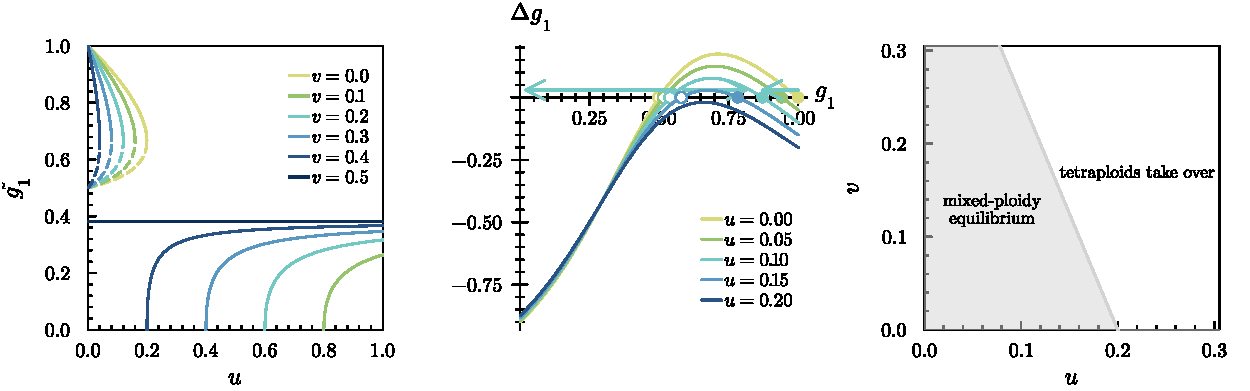
\includegraphics[width=\linewidth]{/home/arthur_z/vimwiki/build/img/2023-10-13/g1diff.pdf}
\caption{
Deterministic mixed-ploidy equilibrium. The left plot shows the stable (solid
lines) and unstable (dashed lines) equilibria for the proportion of haploid
gametes in the gamete pool $g_1$ as a function of $u$ for different values of
$v$. The middle plot shows the relationship between $\Delta g_1 = g_1' - g_1$
and $g_1$. The zeros of this graph are the fixed points of the dynamical system
and are indicated by the hollow (unstable equilibrium) and solid (stable
equilibrium) dots. The rightmost plot shows the region of parameter space where
a stable mixed-ploidy equilibrium exist.
\label{fig:g1diff}}
\end{figure}

\subsection{Stochastic mixed-ploidy model \label{sec:mchain}}

For finite $N$, the basic mixed-ploidy model defines a Markov chain on the
state space $[0..N] \times [0..N]$.
\begin{align}
  p_{ij,kl} = \Pr\{N_2(t+1)=k,& N_3(t+1)=l | N_2(t)=i, N_3(t)=j\} \nonumber \\
    &= \frac{N!}{k!l!(N-k-l)!} p_2^k p_3^l (1-p_2-p_3)^{N-k-l}
\end{align}
where 
\begin{align}
  p_2 &= \left(\frac{i(1-u) + jv}{N(1-u) + (i+j)u + j(2v-1)}\right)^2 \\
  p_3 &= \left(\frac{2(i(1-u) + jv)(N(1-u) + i(2u - 1) + j(u + v - 1))}
    {N(1-u) + (i+j)u + j(2v-1)}\right)^2 
\end{align}
Associating a unique index with each pair $(i,j)$ with $0 \le i,j \le N$, we
can define a transition probability matrix $P$ of dimensions $(N+1)^2 \times
(N+1)^2$ for this Markov chain.

For nonzero $u$ and $v$, the only absorbing state is the one where $N_2 = N_3 =
0$, i.e. the tetraploid cytotype fixes.
All other states are transient, and hence tetraploid fixation occurs with
probability one.
The expected time until fixation may however be extremely long.
Using standard theory for absorbing Markov chains, we can numerically compute
the expected time until fixation $\Ex[T_{\text{fix}}]$ from the transition
probability matrix.
Calculations for the case where $u=v=0.05$ (which are large parameter values
conducive for tetraploid fixation) are shown in \cref{tbl:mchain-ex}.  Clearly,
tetraploid establishment by drift alone requires very small population sizes to
occur at an appreciable rate.
A similar model without triploids has been analyzed by \cite{rausch2005}.

\begin{table}[t]
\caption{
Expected number of generations until fixation of the tetraploid cytotype for
different population sizes, assuming $u=v=0.05$ and an initially diploid
population. \label{tbl:mchain-ex}
}
\begin{tabularx}{\linewidth}{XXXXXX}
\cline{1-6}
$N$ & 10 & 20 & 30 & 40 & 50 \\
\cline{1-6}
$\Ex[T_{\text{fix}}]$ & $5.4 \times 10^3$ & $6.4 \times 10^5$ & 
    $7.9 \times 10^7$ & $9.8 \times 10^9$ & $1.2 \times 10^{12}$ 
\end{tabularx}
\end{table}

\subsection{Expected time to diploid ancestry \label{sec:ttdip}}

Consider a gene sampled from a tetraploid individual in a mixed-ploidy
population at equilibrium and not subjected to selection. Let \(T_4\)
denote the number of generations in the past until such a gene is found
in a diploid ancestor, and let \(T_3\) denote a similar random variable
for a randomly sampled gene from a triploid in the same population.
Assuming the different cytotypes are at their deterministic equilibrium
frequencies \(\pi_2, \pi_3\) and \(\pi_4\) (see sec.~\ref{sec:det},
eq.~\ref{eq:cyteq}), we have the recursive relations \begin{align}
  \Ex[T_4] &= \frac{1}{Z_2}\Big(\pi_2u + (1+\Ex[T_3])\pi_3 v +
    (1+\Ex[T_4])\pi_4(1-u)\Big) \nonumber \\
  \Ex[T_3] &= \frac{1}{3Z_1}\Big(\pi_2(1-u) + (1+\Ex[T_3])\pi_3 v\Big)
  \nonumber
    \\ &\qquad + \frac{2}{3Z_2}\Big(\pi_2 u + (1+\Ex[T_3])\pi_3 v +
      (1+\Ex[T_4])\pi_4(1-u)\Big) \label{eq:ttdip}
\end{align} where \begin{align*}
  Z_1 &= \pi_2(1-u) + \pi_3v \\
  Z_2 &= \pi_2u + \pi_3v + \pi_4(1-u)
\end{align*} (these expressions are straightforwardly modified when more
general \(u_{ij}\) are assumed, see e.g. sec.~\ref{sec:effsize},
eq.~\ref{eq:markovch}). The system in eq.~\ref{eq:ttdip} can be solved
to yield expressions for \(\Ex[T_4]\) and \(\Ex[T_3]\), which are
however rather unwieldy. Again assuming \(v=O(u)\), we obtain to first
order in \(u\) \begin{align*}
\Ex[T_4] &= 1 + u + 2v + O(u^2) \\
\Ex[T_3] &= 1 + \frac{2}{3}(u + 2v) + O(u^2) 
\end{align*} Numerical examples are shown in (fig.~\ref{fig:ttdip}).
Clearly, for plausible parameter values, \(\Ex[T]\) will be very close
to 1. For instance, for \(u=0.05\) and \(v=0.05\) (which are already
rather large values for these parameters), we would have
\(\Ex[T_3] \approx 1.13\) and \(\Ex[T_4] \approx 1.19\).


\begin{figure}
\centering
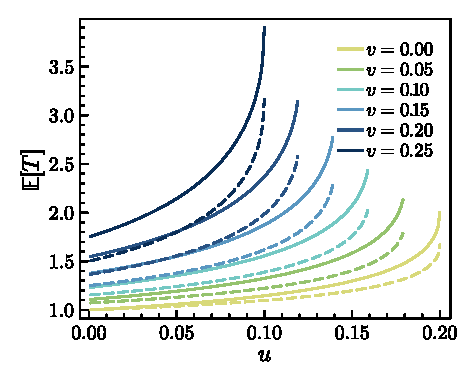
\includegraphics[width=0.5\textwidth]{/home/arthur_z/vimwiki/build/img/2023-10-22/timetodiploidancestord.pdf}
\caption{Expected time to diploid ancestry. The solid lines show
\(\Ex[T_4]\), i.e.~the expected time since being inherited from a
diploid ancestor for a random gene in a tetraploid individual at
equilibrium, for different values of \(v\) (half the triploid
fertility). The dashed lines show \(\Ex[T_3]\), i.e.~the same quantity
for a gene sampled from a triploid. Note that \(\Ex[T]\) blows up
whenever \(u\) and \(v\) exceed their critical value for tetraploid
establishment. \label{fig:ttdip}}
\end{figure}

\subsection{Effective population size of a mixed-ploidy deme \label{sec:effsize}}

\begin{figure}
\centering
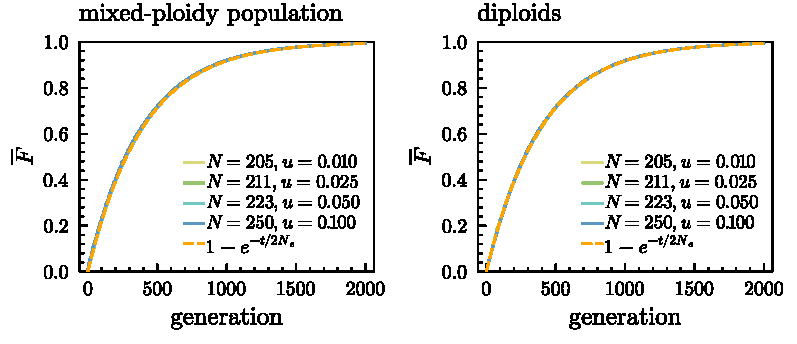
\includegraphics[width=\textwidth]{/home/arthur_z/vimwiki/build/img/2023-10-13/mixedploidy-F-Ne.pdf}
\caption{The evolution of \(\bar{F}\) in the mixed-ploidy population and
in the diploid subpopulation are shown for different values of \(u\) and
associated values of \(N\), keeping \(N_e = (1-2u)N\) constant at 200.
We assume \(u=v\). All lines coincide almost completely and are
indistinguishable from \(1-e^{-t/2N_e}\). Results are shown for
\(\alpha_k=1/6\). As \(\alpha_k\) decreases to 0, \(\bar{F}\) in the
mixed-ploidy population becomes completely indistinguishable from
\(\bar{F}\) in the diploid subpopulation.}\label{fig:fNe}
\end{figure}

We use the approach outlined in \citep{rousset2004} (pp.~153, 157) to
determine the effective size of a randomly mating mixed-ploidy
population. Denote by \(\nu_k(t)\) the probability that the ancestral
lineage of a given gene in the present is found in a individual of
ploidy level \(k\) \(t\) generations in the past, and let
\(\nu(t) = (\nu_2(t)\ \nu_3(t)\ \nu_4(t))\) be the corresponding row
vector. Assuming the population is at cytotype equilibrium
(eq.~\ref{eq:cyteq}), we have 
  \begin{align}
      \nu(t+1) &= \nu(t) P \nonumber \\
               &= \nu(t) \begin{pmatrix}
      \frac{u_{21}}{Z_1}\pi_2 & \frac{u_{31}}{Z_1}\pi_3 & 0 \\
      \left(\frac{u_{21}}{3Z_1} + \frac{2u_{22}}{3Z_2}\right)\pi_2 &
          \left(\frac{u{31}}{3Z_1} + \frac{2u_{32}}{3Z_2}\right)\pi_3 & 
          \frac{2u_{42}}{3Z_2}\pi_4 \\
      \frac{u_{22}}{Z_2}\pi_2 & \frac{u_{32}}{Z_2}\pi_3 & \frac{u_{42}}{Z_2}\pi_4
      \label{eq:markovch}
       \end{pmatrix}
  \end{align}
where we assume, as usual, that tetraploids do not
produce haploid gametes (\(u_{41} = 0\)), and where \begin{align*}
  Z_1 &= u_{21} \pi_2+ u_{31} \pi_3 \\
  Z_2 &= u_{22} \pi_2 + u_{32} \pi_3 + u_{42} \pi_4
\end{align*} At stationarity,
\(\lim_{t\rightarrow \infty} \nu(t) = \nu\), and we have
\(\nu = \nu P\). Hence, the probability that the ancestral lineage of a
given gene in the present is found in an individual of ploidy level
\(k\) in an indefinite past is given by \(\nu_k\), where \(\nu\) is the
left eigenvector of \(P\) associated with the unit eigenvalue. The
effective size of a mixed-ploidy population of size \(N\) can then be
obtained as \[N_e = N\left(\sum_k \frac{\nu_k^2}{\pi_k}\right)^{-1}\]
After plugging in \(\pi\) in accordance with eq.~\ref{eq:cyteq} and
solving the eigenvalue problem, this yields an unwieldy expression in
the \(u_{ij}\). For our usual parameterization where
\(u_{21} = u_{42} = 1-u, u_{22} = u\) and \(u_{31} = u_{32} = v\), and
\(v = O(u)\), we can find that
\[\begin{pmatrix}\nu_2 \\ \nu_3 \\ \nu_4\end{pmatrix} = \begin{pmatrix}
    1-2uv + O(u^3) \\ 2uv + O(u^3) \\ O(u^3)\end{pmatrix}\] and
\[\frac{N_e}{N} = 1 - 2u + O(u^2)\] which yields an excellent fit in
simulations for plausible parameter values (fig.~\ref{fig:fNe}). When
\(v=0\) and \(u < u_c\) (see sec.~\ref{sec:det}), \(N_e = \pi_2N\), as
in that case (i.e.~when triploids are infertile) there can be no gene
flow from tetraploids to diploids. Since we assume the cytotype
composition to be constant, and polyploids are continually formed from
diploids, no gene in a triploid or tetraploid will have any descendants
in the distant future in this case, so that the effective size is just
the diploid fraction of the population.


\subsection{Inbreeding in the mixed-ploidy model}

\subsubsection{Effect of inbreeding on segregation variance in autotetraploids \label{sec:tetinbred}}

In polyploids, the inbreeding coefficient $F_i$ does not suffice to describe
the state of homozygosity in individual $i$.
In tetraploids, for instance, we have five distinct homozygosity states, which
we can symbolically represent as $abcd, aabc, aabb, aaab$ and $aaaa$ (in
general, the number of homozygosity states grows according to the partition
function $(1,2,3,5,7,11,15,22,\dots)$).
Representing the probability of being in these five increasingly homozygous
states as $\delta_1, \dots, \delta_5$, we find that the gametic segregation
variance is reduced by a factor
  $$\phi = \delta_1 + \left(1 - \frac1 6\right) \delta_2 + \left(1 - \frac1
        3\right)\delta_3 + \left(1 - \frac1 2\right) \delta_4$$
which is precisely $1-F_i$, as in diploids (see also \cite{moody1993}).
This shows that we do not need to track the array of homozygosity coefficients
in order to compute the segregation variance in a tetraploid family, but only
require the inbreeding coefficients of the parents.
This is a consequence of the fact that, in tetraploids, gametes are diploid.
Similar considerations apply to triploids if we only model haploid and diploid
gametes.
For higher gametic ploidy levels, one would need to track higher order identity
coefficients in polyploids, which is intractable in general \citep{barton2023}.

\subsubsection{Recursions for inbreeding coefficients in the mixed-ploidy model}

Denoting the parents of individual $i$ by $k$ and $l$, the recursion for the
inbreeding coefficients in an autotetraploid population is
\begin{align}
    F_i &= \frac1 6 (F_k^\ast + F_l^\ast + 4\Phi_{kl}) \label{eq:rectet}
\end{align}
where $F_k^\ast = \alpha_4 + (1-\alpha_4)F_k$.
The recursion follows from considering three cases:
either (1) the two genes sampled in individual $i$ both came from the gamete
contributed by parent $k$, which happens with probability $1/6$, in which case
they are IBD with probability $F_k^\ast$; or (2) as in (1) but from parent $l$; or
(3) with probability $2/3$ the two genes came from different gametes, in which
case they are IBD with probability $\Phi_{kl}$ (the coancestry coefficient for
individuals $k$ and $l$).

There is little difficulty in extending the recursions for diploids
\citep{barton2017} and autotetraploids (\cref{eq:rectet}) to the mixed-ploidy
case. 
Denoting the parents of individual $i$ by $k$ and $l$, the recursion for the
inbreeding coefficients in the mixed-ploidy case becomes
\begin{align}
    F_i &= \Phi_{kl} & \text{if } & c_i = 2 \nonumber \\ 
    F_i &= \frac{1}{3}\left(F_k^\ast + 2\Phi_{kl}\right) & \text{if } 
        & c_i = 3, g_k = 2, g_l = 1 \nonumber \\ 
    F_i &= \frac{1}{3}\left(F_l^\ast + 2\Phi_{kl}\right) & \text{if } 
        & c_i = 3, g_k = 1, g_l = 2 \nonumber \\ 
    F_i &= \frac1 6 (F_k^\ast + F_l^\ast + 4\Phi_{kl}) & \text{if } & c_i = 4
\end{align}
where $F_k^\ast = \alpha_{c_k} + (1-\alpha_{c_k})F_k$, as in the
autotetraploid model.
The recursion for the coancestry coefficients in is given by
\begin{align}
    \Phi_{ii} &= \frac{1}{c_{i}} \left(1 + (c_i-1)F_i\right) \nonumber \\
    \Phi_{ij} &= \sum_k \sum_l P_{ik}P_{jl} \Phi_{kl} & i \ne j 
    \label{eq:coancestry}
\end{align}
where the sums are over individuals in the parental population, and where
$P_{ik} \in \{0, \frac1 3, \frac1 2, \frac2 3, 1\}$ is the probability that a
gene copy in $i$ is derived from parent $k$.


\subsection{Mixed-ploidy infinitesimal model}

\subsubsection{Discrete locus model and variance scaling \label{sec:scaling}}

Consider an $L$-locus additive model, with two alleles (0 and 1) at each locus.
For a $k$-ploid individual, let $X_{i,j}$ be the allele at homolog $j$ of locus
$i$.
We assume the trait value is determined by
\begin{equation}
  z = \sum_{i=1}^L\sum_{j=1}^k a_{i,k} X_{i,j}
\end{equation}
Where $a_{i,k}$ is the allelic effect of the 1 allele at locus $i$ in
$k$-ploids.
The genetic variance at HWLE in $k$-ploids ($\tilde{V}_{z,k}$) will then be
\begin{equation}
  \tilde{V}_{z,k} = k\sum_{i=1} a_{i,k}^2 p_iq_i = kV_{x,k}
\end{equation}
where we refer to $V_{x,k}$ as the variance associated with a haploid genome in
$k$-ploids at HWLE.
Note that we also have $\tilde{V}_{z,2} = 2V_{x,k} = 2V$, where $V$ is the
segregation variance in the diploid population.

We now assume $a_{i,k} = \beta_k a_{i,2}$, i.e. allelic effects in $k$-ploids
are as in diploids, but scaled by a factor $\beta_k$.
This implies that
\begin{equation}
  \frac{\tilde{V}_{z,k}}{\tilde{V}_{z,2}} 
  = \frac{kV_{x,k}}{2V_{x,2}} = \frac{k}{2} \beta_{k}^2
\end{equation}
and hence also that $V_{x,k} = \beta_k^2 V_{x,2} = \beta_k^2 V$.
These relations will also hold in the infinitesimal limit.
Below, we derive the segregation variance expressions for the different meiotic
processes in the mixed-ploidy models in terms of the $V_{x,k}$.
Using the relationships outlined here, we will then be able to express all the
required variances in terms of $V$.

Note that under the above assumptions, not only the variance is rescaled, but
also the expected value of offspring within a family.
Specifically, for a $k$-ploid offspring of parental pair $i$ and $j$, where the
gamete coming from $i$ is $g_i$-ploid and the other gamete $g_j$-ploid, we have
\begin{equation}
  \Ex[Z_{ij}] = \beta_k \left(\frac{g_i}{c_i}\frac{z_i}{\beta_{c_i}} + 
    \frac{g_j}{c_j}\frac{z_j}{\beta_{c_j}}\right)
\end{equation}
where $c_i$ is the ploidy level of individual $i$.
Here we rescale the parental trait values to the diploid scale by dividing by
$\beta_{c_i}$, sum the expected rescaled gametic values, and rescale to the
offspring ploidy level.

\subsubsection{Segregation variance \label{sec:segvar}}

Consider a single locus in a population of $k$-ploids, and let $X_1,\dots,X_k$
denote a random genotype at this locus, where $X_i$ is the additive genetic
value of the allele on homolog $i$.
The variance in gametic values $Y$ produced by some meiotic process can be
decomposed as 
\begin{equation}
  \Var[Y] = \underbrace{\Ex\left[\Var[Y|X_1, \dots, X_k]\right]}_{\text{segregation variance}} 
    + \underbrace{\Var\left[\Ex[Y|X_1, \dots, X_k]\right]}_{\text{population
variation}}
\label{eq:eve}
\end{equation}
We use this relationship to derive the segregation variance for a given meiotic
process.

As an example, consider ordinary diploid meiosis at a single locus, where a
diploid produces a haploid gamete. $Y$ is a random haploid gamete sampled from the
population, and $\Var[Y] = \Var[X] = v_x$, where $X$ is a a randomly sampled
gene from the population and $v_x$ is the variance in additive genetic values
at the locus.
We have
  $$\Var[\Ex[Y|X_1,X_2]] = \Var\left[\frac{X_1 + X_2}{2}\right] = \frac{v_x}{2}$$
Using \cref{eq:eve}, we can then find the segregation variance
  $$\Ex[\Var[Y|X_1,X_2]] = v_x - \frac{v_x}{2} = \frac{v_x}{2}$$
Summing over $L$ independent loci, we find the gametic segregation variance in
diploids (which is halve the zygotic segregation variance $V$, by definition) as
  $$V_{S(2,1)} = \frac{V}{2} = \sum_{i=1}^L \frac{v_{x,i}}{2} = \frac{V_{x,2}}{2}$$
and hence $V=V_{x,2}$, where $V_{x,2}$ is as defined in \cref{sec:scaling}.
This will hold in the infinitsimal limit, where $L$ becomes very large and
$v_x$ smaller and smaller.

Below, we derive the segregation variance associated with haploid and diploid
gamete production in the three cytotypes of the mixed-ploidy population.
We use \cref{eq:eve} to do this, and express the segregation variance for a
$k$-ploid individual producing an $l$-ploid $V_{S(k,l)}$ in terms of the
variance $V_{x,k}$ associated with a haploid genome in a (hypothetical)
$k$-ploid reference population at HWLE. Using the scaling assumptions above,
i.e. $V_{x,k} = \beta_k^2 V$, we can then express all segregation variances in
terms of the diploid segregation variance in the reference population $V$.

\paragraph{Meiosis in autotetraploids.}

When an autotetraploid forms quadrivalents during prophase I, a form of
'internal inbreeding' may occur as a result of the phenomenon called
\textit{double reduction} (see e.g. \cite{lynch1998} p. 57).
Double reduction happens when, as a result of recombination, replicated gene
copies on sister chromatids move to the same pole during anaphase I, as
illustrated in \cref{fig:dr}.
In the example shown in \cref{fig:dr}, one of the four generated gametes is $AA$,
which would not occur in the ordinary bivalent meiosis, because in that case,
paired chromosomes (involved in cross-overs) are separated during anaphase I.
The frequency of double reduction at a locus in the presence of multivalent
formation is hence determined by the frequency at which that locus is involved
in a cross-over (which depends on the distance to the centromere), and has an
upper bound at $1/6$ \citep{stift2008}.

When double reduction occurs, an $ABCD$ genotype would generate 10 distinct
gametes, as opposed to 6 in when chromosomes form bivalents. As a result, the
segregation variance is increased by double reduction.
For a random genotype $X_1X_2X_3X_4$, we can find the gametic segregation
variance contributed by a locus when double reduction happens as
\begin{align*}
    \Ex[\Var[Y|X_1,X_2,X_3,X_4]] &= \Var[Y] - \Var[\Ex[Y|X_1,X_2,X_3,X_4]] \\
        &= \Var[2X] - \Var\left[\frac1 4 (2X_1 + 2X_2 + 2X_3 + 2X_4)\right] \\
        &= 4v_x - \frac{1}{4}4v_x 
        = 3v_x
\end{align*}
where $X$ denotes the additive effect of a random allele at the locus drawn from the reference
population and $v_x = \Var[X]$.
In the absence of double reduction we have
\begin{align*}
    \Ex[\Var[Y|X_1,X_2,X_3,X_4]] 
        &= 2\Var[X] - \Var\left[\frac1 6 \sum_{i=1}^3 \sum_{j=i+1}^4(X_i+X_j)\right]
        = v_x
\end{align*}
Assuming that the probability of double reduction at any locus is $\alpha_4$,
and summing over independent loci, we find that the gametic segregation
variance in the presence of double reduction should be
\begin{equation}
V_{S(4,2)} = (1-\alpha_4)V_{x,4} + 3\alpha_4 V_{x,4} = V_{x,4}(1+2\alpha_4).
\label{eq:dr}
\end{equation}
where, again, $V_{x,4}$ is as defined in \cref{sec:scaling}.

\begin{figure}
\begin{center}
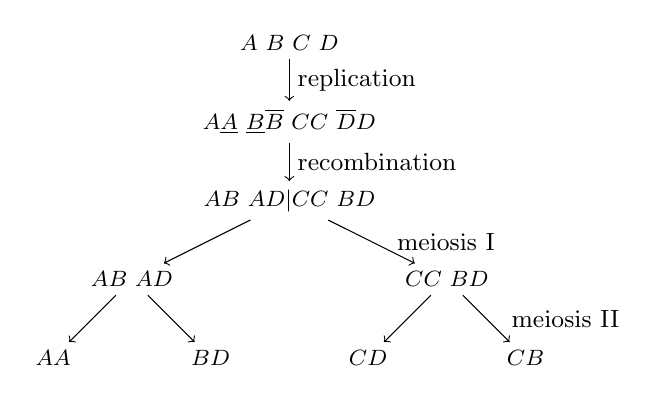
\begin{tikzpicture}
\footnotesize
\node (n1) at (0, 5) [] {$A\ B\ C\ D$};
\node (n2) at (0, 4) [] {$A\underline{A}\ \underline{B}\overline{B}\ CC\ \overline{D}D$};
\node (n3) at (0, 3) [] {$AB\ AD | CC\ BD$};
\node (n4) at (-2, 2) [] {$AB\ AD$};
\node (n5) at ( 2, 2) [] {$CC\ BD$};
\node (n6) at (-3, 1) [] {$AA$};
\node (n7) at (-1, 1) [] {$BD$};
\node (n8) at ( 3, 1) [] {$CB$};
\node (n9) at ( 1, 1) [] {$CD$};
\draw[->] (n1) -- (n2) node [right,midway] {\small replication};
\draw[->] (n2) -- (n3) node [right,midway] {\small recombination};
\draw[->] (n3) -- (n4);
\draw[->] (n3) -- (n5) node [right,midway] {\small \ \ meiosis I};
\draw[->] (n5) -- (n8) node [right,midway] {\small \ \ meiosis II};
\draw[->] (n5) -- (n9);
\draw[->] (n4) -- (n6);
\draw[->] (n4) -- (n7);
\end{tikzpicture}
\end{center}
\begin{caption}{
Schematic illustration of a meiotic division in an autotetraploid leading to
double reduction at a locus with genotype $ABCD$.
Two recombination events are assumed to occur at the locus (denoted by the
bars).
\label{fig:dr}
}\end{caption}
\end{figure}


\paragraph{Unreduced gamete formation in diploids.}

\begin{figure}
\begin{center}
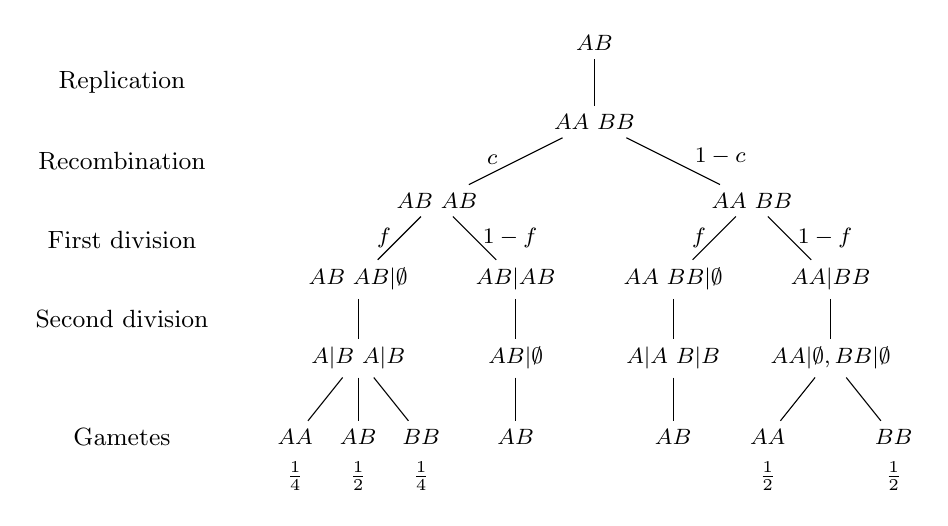
\begin{tikzpicture}
\footnotesize
\node (rep) at (-6, 4.5) [] {\small Replication};
\node (rep) at (-6, 3.5) [] {\small Recombination};
\node (rep) at (-6, 2.5) [] {\small First division};
\node (rep) at (-6, 1.5) [] {\small Second division};
\node (rep) at (-6, 0)   [] {\small Gametes};
\node (Aa)  at (0, 5) [] {$AB$};
\node (AAaa)  at (0, 4) [] {$AA\ BB$};
\node (rAaAa) at (-2, 3) [] {$AB\ AB$};
\node (rAAaa) at ( 2, 3) [] {$AA\ BB$};
\path (Aa) edge (AAaa);
\path (AAaa) edge node[near end, above] {$c$} (rAaAa) ;
\path (AAaa) edge node[near end, above] {\qquad $1-c$} (rAAaa);

\node (fdr11) at (-3, 2) [] {$AB\ AB | \emptyset$};
\node (fdr12) at (-3, 1) [] {$A|B\  A|B$}; 
\node (AA) at (-3.8,0) [] {$AA$};
\node (p1) at (-3.8,-0.5) [] {$\frac{1}{4}$};
\node (Aa) at (-3,0) [] {$AB$};
\node (p2) at (-3,-0.5) [] {$\frac{1}{2}$};
\node (aa) at (-2.2,0) [] {$BB$};
\node (p2) at (-2.2,-0.5) [] {$\frac{1}{4}$};
\path (fdr12) edge (AA);
\path (fdr12) edge (Aa);
\path (fdr12) edge (aa);
\path (fdr11) edge (fdr12);
\path (rAaAa) edge node[left] {$f$} (fdr11);

\node (sdr11) at (-1, 2) [] {$AB | AB$}; 
\node (sdr12) at (-1, 1) [] {$AB | \emptyset$}; 
\node (Aa2) at (-1,0) [] {$AB$};
\path (sdr12) edge (Aa2);
\path (sdr11) edge (sdr12);
\path (rAaAa) edge node[right] {$1-f$} (sdr11);

\node (fdr21) at (1,2) [] {$AA\ BB|\emptyset$};
\node (fdr22) at (1,1) [] {$A|A\ B|B$};
\node (Aa3) at (1,0) [] {$AB$};
\path (rAAaa) edge node[left] {$f$} (fdr21);
\path (fdr21) edge (fdr22);
\path (fdr22) edge (Aa3);

\node (sdr21) at (3, 2) [] {$AA | BB$};
\node (sdr22) at (3, 1) [] {$AA| \emptyset, BB|\emptyset$};
\node (AA4) at (2.2,0) [] {$AA$};
\node (p1) at (2.2, -0.5) [] {$\frac{1}{2}$};
\node (aa4) at (3.8,0) [] {$BB$};
\node (p2) at (3.8, -0.5) [] {$\frac{1}{2}$};
\path (rAAaa) edge node[right] {$1-f$} (sdr21);
\path (sdr21) edge (sdr22);
\path (sdr22) edge (AA4);
\path (sdr22) edge (aa4);
\end{tikzpicture}
\begin{caption}{
Schematic representation of the different pathways for unreduced gamete
formation in diploids and their different outcomes.
\label{fig:udip}
}\end{caption}
\end{center}
\end{figure}

The mechanisms of unreduced gamete formation do not necessarily lead to a
faithful transmission of the complete diploid genome.
Unreduced gametes are formed in two ways, depending on the meiotic abberation
that leads to their origin: (1) first division restitution (FDR) of (2) second
division restitution (SDR) \citep{bretagnolle1995,storme2013}.
Consider a locus in a diploid with two distinct genes $A$ and $a$. Assume
recombination happens with probability $c$ and that conditional on unreduced
gamete formation, formation is due to FDR with probability $f$ while it is due
to SDR with probability $1-f$.
The different unreduced gametes that are formed are represented schematically
in \cref{fig:udip}.
Writing the genotype at a locus in the diploid parent as $X_1X_2$, with allelic
effects $X_1$ and $X_2$, the genotypic value of an unreduced gamete at this
locus will be
$$Y = \begin{cases}
    2X_1 & \text{w.pr.  } \alpha_2/2 \\
    2X_2 & \text{w.pr.  } \alpha_2/2 \\
    X_1 + X_2 & \text{w.pr.  } 1-\alpha_2 
    \end{cases}$$
where $\alpha_2 = 1 - f - c + \frac{3}{2}cf$ is the probability that two copies
of the same gene end up in a diploid gamete produced by a diploid individual
(see the diagram in \cref{fig:udip}). 
Conditional on the latter event, we get
\begin{align*}
\Ex[\Var[Y|X_1,X_2]] &= \Var[Y] - \Var[\Ex[Y|X_1,X_2]] \\
    &= \Var[2X] - \Var\left[\frac{1}{2}(2X_1 + 2X_2)\right] \\
    &= 2v_x
\end{align*}
Conditioning on the complementary event, all gametes have genetic value
$Y = X_1+X_2$, so that the segregation variance is 0.
Summing across independent loci, we have $V_{S(2,2)} = 2\alpha_2 V_{x,2}$.


\paragraph{Meiosis in triploids.}

Triploids, when viable, may be important for the dynamics of mixed-ploidy
populations due to the formation of a so-called triploid bridge.
The formation of triploids presents no immediate issues, we simply need to
track the segregation variance contributions from both donor gametes, and
relate these to $V_{0,3}$.
Sexual reproduction in triploids is however more complicated.
There are no known mechanisms to coordinate the assortment of chromosomes in
for instance a haploid and diploid gamete, and meiosis, if it happens, usually
results in aneuploid gametes \citep{ramsey1998}.

Experimental results indicate that, at least in yeast, triploids usually form
trivalents and undergo recombination, after which each trivalent is randomly
assorted in the daughter cells, some receiving one, others two copies of a
given chromosome \citep{charles2010}.
In the absence of gametic nonreduction, the probability
of obtaining euploid gametes (two diploid and two haploid gametes) from such 
a process is $(1/2)^n$, where $n$ is the number of chromosomes. If the number
of chromosomes is small this is not negligible, for instance in
\textit{Arabidopsis thaliana} we would have $(1/2)^5 \approx 0.03$, which is of
the same order as the unreduced gamete formation rate.
Unreduced (triploid) gametes may also be produced and important for the
dynamics of mixed-ploidy populations \citep{ramsey1998}.
However, they generate additional difficulty, since in order to compute the
contributed variance under inbreeding, we would need an additional identity
coefficient recording the probability that three genes are IBD at a locus.
We will hence ignore the possibility of unreduced gamete production in
triploids.
We note that, on the supposition that diploid gametes are produced by random
assortment of chromosomes in a haploid and diploid gametes, $\alpha_3 \le 1/4$.

When a triploid produces a haploid gamete, we get as segregation variance at a
single locus
\begin{align*}
  \Ex[\Var[Y|X_1,X_2,X_3]] &= \Var[Y] - \Var[\Ex[Y|X_1,X_2,X_3]] \\
    &= v_x - \Var\left[\frac{1}{3}\left(X_1 + X_2 + X_3\right)\right] \\ 
    &= v_x - \frac{1}{9}3v_x = \frac{2}{3}v_x
\end{align*}
Summing over many loci, we have $V_{S(3,1)} = \frac{2}{3}V_{x,3}$.
When a triploid produces a diploid gamete, we assume there is, as in diploids
and tetraploids, a probability $\alpha_3$ that the same gene copy ends up twice
in the gamete.
Conditional on this happening, we have
\begin{align*}
  \Ex[\Var[Y|X_1,X_2,X_3]] &= \Var[Y] - \Var[\Ex[Y|X_1,X_2,X_3]] \\
    &= \Var[2X] - \Var\left[\frac{1}{3}\left(2X_1 + 2X_2 + 2X_3\right)\right] \\
    &= 4V_x - \frac{4}{9}3V_x = \frac{8}{3}V_x
\end{align*}
Conditional on this \textit{not} happening, 
\begin{align*}
  \Ex[\Var[Y|X_1,X_2,X_3]] &= \Var[Y] - \Var[\Ex[Y|X_1,X_2,X_3]] \\
    &= 2V_x - \Var\left[\frac{1}{3}\left((X_1+X_2) + (X_1+X_3) +
      (X_2+X_3)\right)\right] \\
    &= 2V_x - \frac{4}{9}3V_x = \frac{2}{3}V_x
\end{align*} 
Putting this together and summing over many loci, the segregation variance for
a diploid gamete from a triploid individual would be
  $$V_{S(3,2)} = \frac{8}{3}V_{x,3}\alpha_3 + \frac{2}{3}V_{x,3} (1-\alpha_3) 
            = \frac{2}{3}V_{x,3}(1 + 3\alpha_3)$$ 

The different expressions for the gametic segregation variance in the
mixed-ploidy model, adjusted for inbreeding, are summarized in
\cref{m-tbl:segvar} in the main text.


\bibliographystyle{abbrvnat}
\bibliography{/home/arthur_z/vimwiki/bib.bib}
\end{document}
